\documentclass{beamer}
\usepackage[T1]{fontenc}
\usepackage[utf8]{inputenc}
\usepackage{lmodern}
\usepackage{textcomp}
\usepackage{lastpage}
%
\title{Towards Socially Responsible AI: Cognitive Bias-Aware Multi-Objective Learning
}
%
\begin{document}
\normalsize
\maketitle
%
\begin{frame}{Introduction}
%
\begin{itemize}
\item
 This social discrimination has manifested itself in different forms, identified by a wide range of different characteristics, such as gender, ethnicity, religion and caste, among others. Scientific and technological revolution has played a pivotal role in mitigating social biases and prejudices to a large extent in modern human society. To corroborate this point,
\item
existing studies have shown that word embedding reflects the gender stereotypes present in large volumes of text \citep{Bolukbasi:2016,manzini-etal-2019}, e.g. \emph{men are more likely to be computer programmers while women are more likely to be home-makers}. A possibility in feature-based models is to manually intervene and leave out the features that could lead to biased predictions for a task, e.g. the New York Police Department (NYPD) refrains from using the \emph{race} of a person to predict the risks of future crimes \citep{ProPublica}. \begin{comment}
\item
\paragraph{Our Contributions.} Existing debiasing studies typically involve one of the following broad classes of techniques. Specifically, we propose a generic approach to first quantify and then reduce bias \emph{jointly} against a number of secondary \emph{social identity} attributes (e.g. gender and ethnicity) in a \emph{classification} task involving a single \emph{primary} attribute (e.g. predicting emotions, such as fear, anger etc. from a piece of text).
\end{itemize}
\end{frame}
%
\begin{frame}{Introduction}
%
\begin{figure}[t]
    \centering
    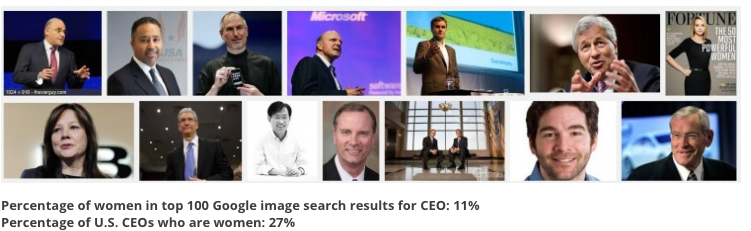
\includegraphics[width=.75\columnwidth]{ceo.png}
    
\includegraphics[width=.24\columnwidth]{qc.png}
    \caption{Examples of social bias in existing AI systems: `Google Image Search' under-representing women as CEOs (left), and `Google query completion' prioritizing \emph{appearance} over \emph{filmography} for a popular female actor (right).}
    \label{fig:bias-in-existing-AI-tools}
\end{figure}
\end{frame}
%
\end{document}
